%2345678901234567890123456789012345678901234567890123456789012345678901
\chapter{RADAMS: Curation, Packaging and Policy} % (fold)
\label{cha:radams_curation_packaging_and_policy}
	
	In this chapter we will follow with our detailed description
	of the RA\-DAMS, making emphasis on several classes which were
	introduced in the ObsDM, but which where not actually defined.
	
	These classes are the Curation class, the Packaging class,
	and the Policy class. There is still another class introduced
	by the ObsDM pending of definition, the Provenance class,
	but due to its relevance we will devote two separate chapters
	to it: one to the concept of Data Provenance in e-Science,
	and one to the actual implementation of Data Provenance in
	the RADAMS.
	
	\section{Curation} % (fold)
	\label{sec:curation}
		
		\attributedquote{
			\dictionarydef
				{curator}
				{noun}
				{
					\begin{itemize}
						\item a keeper or custodian of a museum or
						other collection.
					\end{itemize}
				}
			\dictionarydef
				{curate}
				{verb [trans.] (usu. \textbf{be curated})}
				{
					\begin{itemize}
						\item select, organize, and look after the
						items in (a collection or exhibition):
						\emph{both exhibitions are curated by the
						museum's director.}
					\end{itemize}
				}
			
		}
		{The New  Oxford American Dictionary, \emph{2nd Edition}}
		
		\noindent If we conceive sets of astronomical observations
		(for instance, a particular observation program, a whole
		sky survey, et cetera) as \emph{collections \emph{or}
		exhibitions}, we can also generalise the VO concept (or any
		other data based e-Infrastructure) as a special kind of
		digital \emph{museum}.
		
		In that case, the definitions above point us to the fact
		that, for digital data collections, Curation is related to:
		
		\begin{itemize}
			\item the final decision on what elements do finally
			enter the collection, and those who do not; that is,
			which digital copies of data will be offered as members
			of a particular dataset.
			
			\item the organisation on how the data collection is
			finally presented; that is, which services will be
			offered which contain a particular dataset, and which
			will be the access end-points to them.
			
			\item the care-taking of the items put in that
			collection; that is, keeping the datasets accessible,
			and updated if the archive admits updating.
		\end{itemize}
		
		So, the most important things the Curation data model has
		to deal with are grouping together all mandatory metadata for
		resources to be published in a VO Registry. We will make use
		of several additional classes in order to deal with Curation
		specifics.
		
		One of the first sources for data curation in the first
		place is the \emph{Resource metadata for the
		VO}~\cite{IVOA-Resource-Registry-WG:2007rm} IVOA
		Recommendation. VO Registry entries are actually the
		\emph{virtual exhibitions} we are exposing by means of
		VO data access protocols, so being able to know who
		curates, who is responsible for the \emph{exhibition} is
		one of the needs for the Registry. 
		
		The Curation data model groups all metadata mandatory for
		resources to be published by a VO Registry. Several
		additional classes are needed for particular instances of
		data. Such classes and metadata are described by “Resource
		Metadata for the VO”, an IVOA Recommendation
		\cite{2004ASPC..314..273H}. Figure
		\ref{figCurationDataModel} encompasses all classes related
		to metadata for curation.
		
		\begin{figure}[tbp]
			\begin{center}
				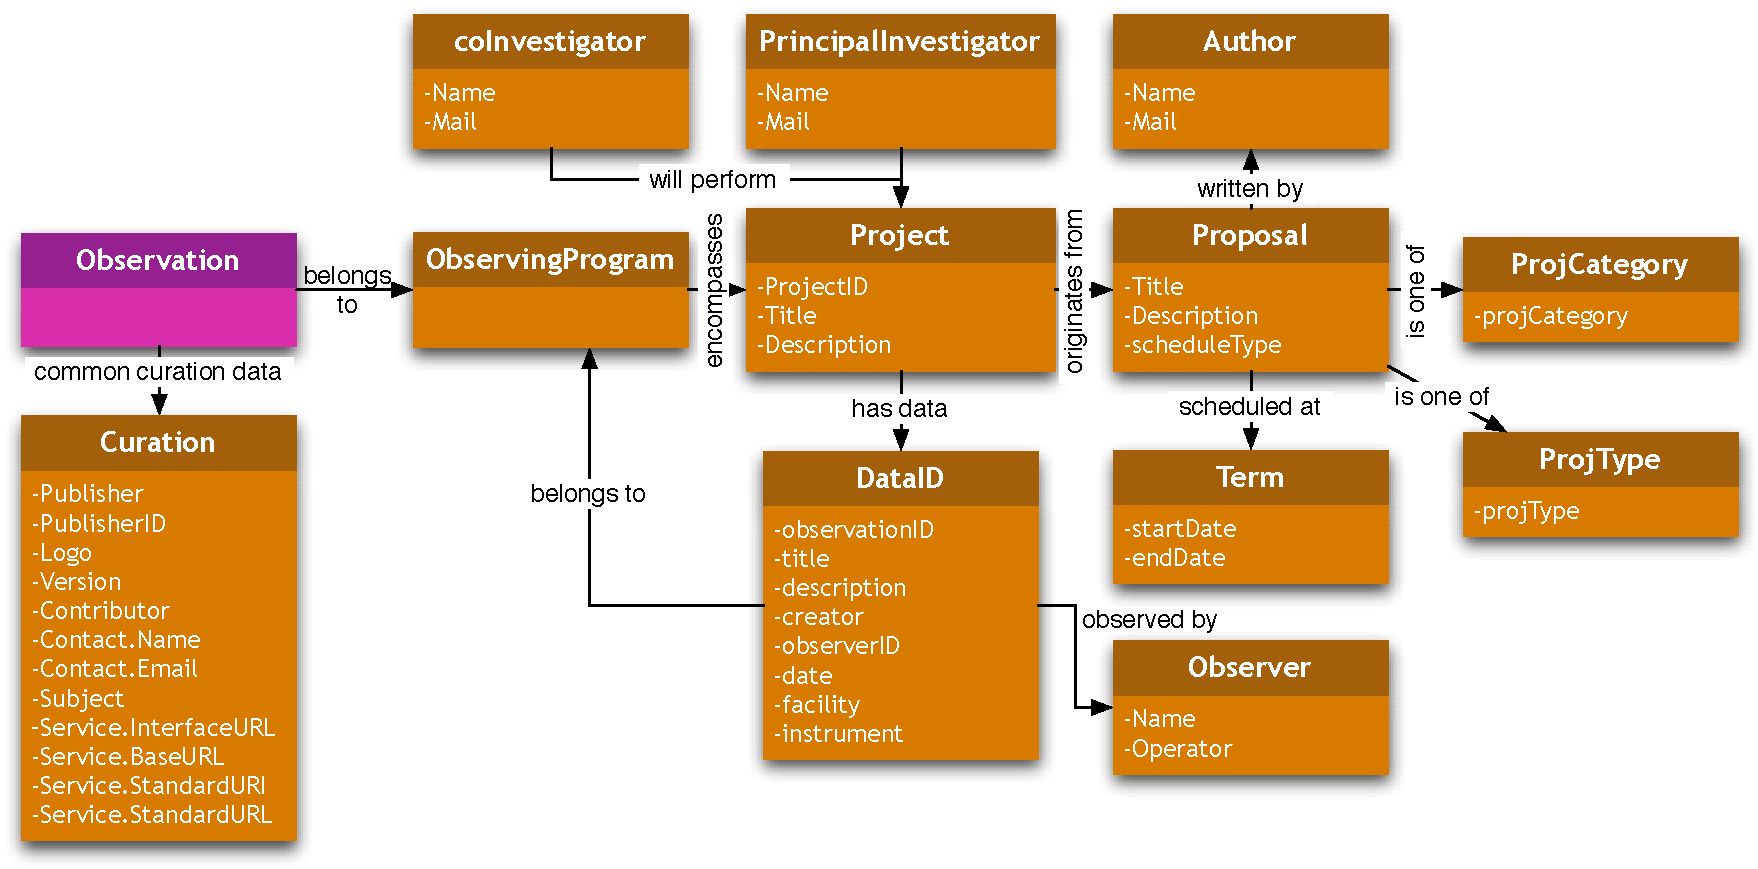
\includegraphics[width=\columnwidth]
				{fig/CurationClass.pdf}
			\end{center}
			\caption[Curation data model]{Curation data model.}
			\label{figCurationDataModel}
		\end{figure}
		
		\begin{description}
			\item[Observation]  The Observation class was
			discussed earlier. All observations are related to a single
			Curation class.

			\item[Curation]  This is the main class that will group
			all curation related metadata with relationships to
			complementary classes such as DataID and the rest.
			It is the same for all data contained in the VO resource
			(archive) being described.

			\item[DataID]  There is an instance of this class for
			each different piece of data stored, or at least for each
			different way to store data. The Spectral Data Model
			advocates for this separation.

			\item[ObservingProgram]  Instances of this class keep
			common information about different observations, describing
			its scientific or technical goals. They also specify which
			is the project and/or proposal to which this observing
			program belongs. This class allows for easy querying by
			project or by common goals, such as maser surveys.

			While there is debate about whether this class belongs to
			the Curation or to the Provenance Data Model, we believe it
			belongs to the Curation Data Model, as it is an
			organisational unit, and in our view it has nothing to do
			with how the data were taken.

			\item[Project]  This class is the main class from an
			organizational point of view. All observations belong to a
			single project through a single proposal. A
			Project instance is related to a collection of
			Proposal instances.

			\item[Proposal]  As stated in the Project
			class, a Project can be divided in a series of
			Proposals. A Proposal instance can be
			related to one or more observations. No observation can be
			related to more than one Proposal instance.

			\item[Author]  An Author instance contains
			information about Proposal authors.

			\item[Observer]  Observer instances represent
			the observer/s assigned to a Proposal. It also
			contains a relationship with a Contact acting as
			the operator for the instrument.

			\item[ProjCategory]  This instance specifies the
			scientific category of the project, from a controlled
			vocabulary; possible values, as specified by the Resource
			Data Model, are: \texttt{instrumental}, \texttt{galactic},
			\texttt{ter\-res\-tri\-al}, \texttt{so\-lar\-Sys\-tem},
			\texttt{ex\-tra\-ga\-lac\-tic}, \texttt{stellar}…

			\item[ProjType] This instance specifies the type of
			observation performed for a particular proposal.
			Possible values are specified by the Resource Data
			Model, and form a controlled vocabulary that we have
			derived from Lamb's, ATNF and NRAO
			proposals~\cite{2006astro.ph..1354, LamPow0310IVOA,
			PreCla0412Device}:
			\texttt{as\-trom\-e\-try},
			\texttt{band\-width\-Syn\-the\-sis},
			\texttt{cir\-cu\-lar\-Po\-lar\-i\-za\-tion},
			\texttt{con\-tin\-u\-um}, \texttt{en\-gi\-neer\-ing},
			\texttt{fill\-er\-Time},
			\texttt{high\-Time\-Res\-o\-lu\-tion},
			\texttt{im\-ag\-ing}, \texttt{in\-stru\-men\-tal},
			\texttt{lin\-e\-ar\-Po\-lar\-i\-za\-tion},
			\texttt{map\-ping}, \texttt{mon\-i\-to\-ring},
			\texttt{mo\-sa\-ic}, \texttt{mul\-ti\-beam},
			\texttt{point\-Source}, \texttt{phased\-Ar\-ray},
			\texttt{po\-lar\-im\-e\-try}, \texttt{snap\-shot},
			\texttt{so\-lar}, \texttt{spec\-tros\-copy},
			\texttt{sur\-vey}, \texttt{time\-Bin\-ning}.
			
			\item[Term] Specifies start and end dates (ISO dates,
			with time stamp) for the proposal \emph{observing term}
			or \emph{scheduling block}.
		\end{description}
		
		
		\invisiblenote{
		Describe the linking of the ObsData identifier with
		Curation; Curation should be linked from ObsData, as there
		will be a many to one relationship typically for most
		observations, but if several services are built with
		different characteristics (for instance, a most isolated
		galaxies catalogue from a more general galaxy catalogue).}
		
		\invisiblenote{
		\newcommand{\ivoacpigurl}[0]
		{http://www.ivoa.net/cgi-bin/twiki/bin/view/IVOA/IvoaCP}
		Integrate the existence of the IVOA Data Curation and
		Preservation interest group\urlnote{\ivoacpigurl}.}
		
	% section curation (end)
	
	\section{Policy} % (fold)
	\label{sec:policy}
		\attributedquote{
			\dictionarydef
				{policy}
				{noun}
				{
					\begin{itemize}
						\item a course or principle of action
						adopted or proposed by a government, party,
						business, or individual.
						
						\item \textsf{archaic} prudent or expedient
						conduct or action.
					\end{itemize}
				}
		}
		{The New  Oxford American Dictionary, \emph{2nd Edition}}
		
		\noindent
		The general definition above translates into the VO as
		\emph{data access policy}, and could be defined as
		the expedient action of granting or denying access to
		data following some principles proposed by data
		providers. Those principles take into account who is
		responsible for the data generation, for the data curation,
		and their relationship to the user trying to access the
		data.
		
		Moreover, those principles (policies) can change from
		institution to institution, and also for different datasets
		curated by those institutions. Hence, we need to generalise
		a way to specify those different policies, both regarding
		the different users' relationships with the datasets, and
		the different ways to implement policies, from
		\emph{everything is accessible}, to \emph{PI's eyes only}.
		
		\invisiblenote
		{\textbf{Rewrite this paragraph coming from the DEA
			Details chapter and Policy appendix to accommodate
			to the chapter style.}}
			
		The role of the Policy data model is to allow for very
		different policies to be applied to the data. In the case
		of a VO archive where the data are not immediately
		available (they have to be manually incorporated to the
		archive), Policy can become simpler, as in \emph{everything
		in the archive is available for everyone}.
		Figure~\ref{figPolicyDataModel} shows the different classes
		needed to characterise the archive policy.
			
		\begin{figure}[tbp]
			\begin{center}
				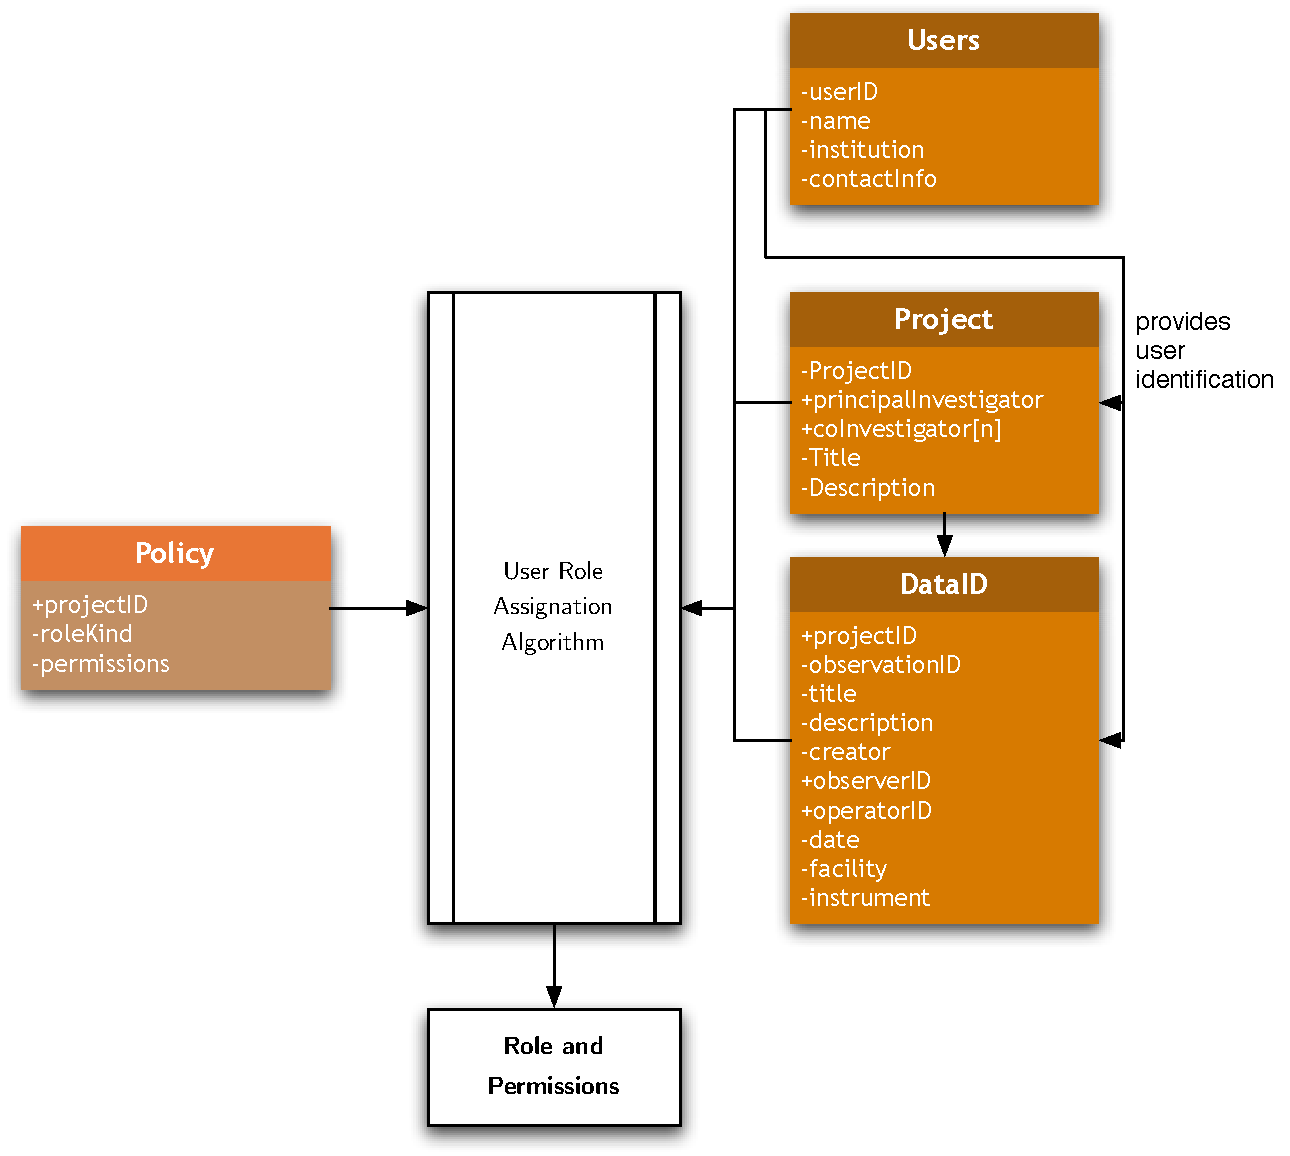
\includegraphics[width=\columnwidth]
				{fig/Policy-DM}
			\end{center}
			\caption[Policy data model]
				{Policy data model, with role and permissions.}
			\label{figPolicyDataModel}
		\end{figure}
		
		Policy instances attached to raw data shall need to
		identify the different roles of agents ---not just people,
		but software packages too--- accessing the archive, and give
		them appropriate access rights to pieces of data.
		
		 In the case of the Robledo Archive, the policy to be
		implemented should be the standard NRAO policy: 18 months
		since the end of the observations. Such a simple policy is
		better accomplished by not entering data into the archive
		until the proprietary period has expired.
		
		 A more flexible solution would make use of an array of
		permissions by role, where roles are derived from the
		relationship between the principal investigator and/or the
		observer, and observatory staff.
		
		 Such roles would be chosen from a controlled vocabulary
		(\texttt{prin\-ci\-pal\-In\-ves\-ti\-ga\-tor},
		\texttt{observer}, \texttt{co\-Inves\-tiga\-tor},
		\texttt{observatory\-Staff}, \texttt{none}); those roles
		are derived from user/project relationships, so that people
		not belonging to the observatory, and which have nothing to
		do with the project, would default to \texttt{none}.
		
		 Each project in the archive should have, at least, an
		explicit policy of what is allowed for some with none
		relationship with the Principal Investigator, and people
		with \texttt{prin\-ci\-pal\-In\-ves\-ti\-ga\-tor} roles
		have all access rights to the archive; people with roles
		other than \texttt{prin\-ci\-pal\-In\-ves\-ti\-ga\-tor}
		would fallback to the \texttt{none} role, if their role’s
		permissions are not explicitly declared.
		
		We will use Policy, Users and ObsData metadata in order to
		select the corresponding role for the agent just logged in.
		Figure~\ref{figPolicyRoles} shows the flow diagram for the
		role selection.
		
 		Policy metadata and attributes are specified in Table
		\ref{tabPolicyMetadata}, but also we will specify a subset
		of Curation attributes needed for successful Policy
		attribution.
		
		 We are also considering of establishing with the Policy
		data model data-oriented policies, instead of
		user-oriented. Data-oriented policies allow each
		datum ---possibly by means of the DataID or Project
		classes---
		to be searched and found, but no additional information, or
		only partial information —possibly having to do with the
		owner of the datum— can be retrieved, depending on the data
		policy in place. This needs at least an additional
		attribute in the DataID class.
		
		\begin{figure}[tbp]
		\begin{center}
		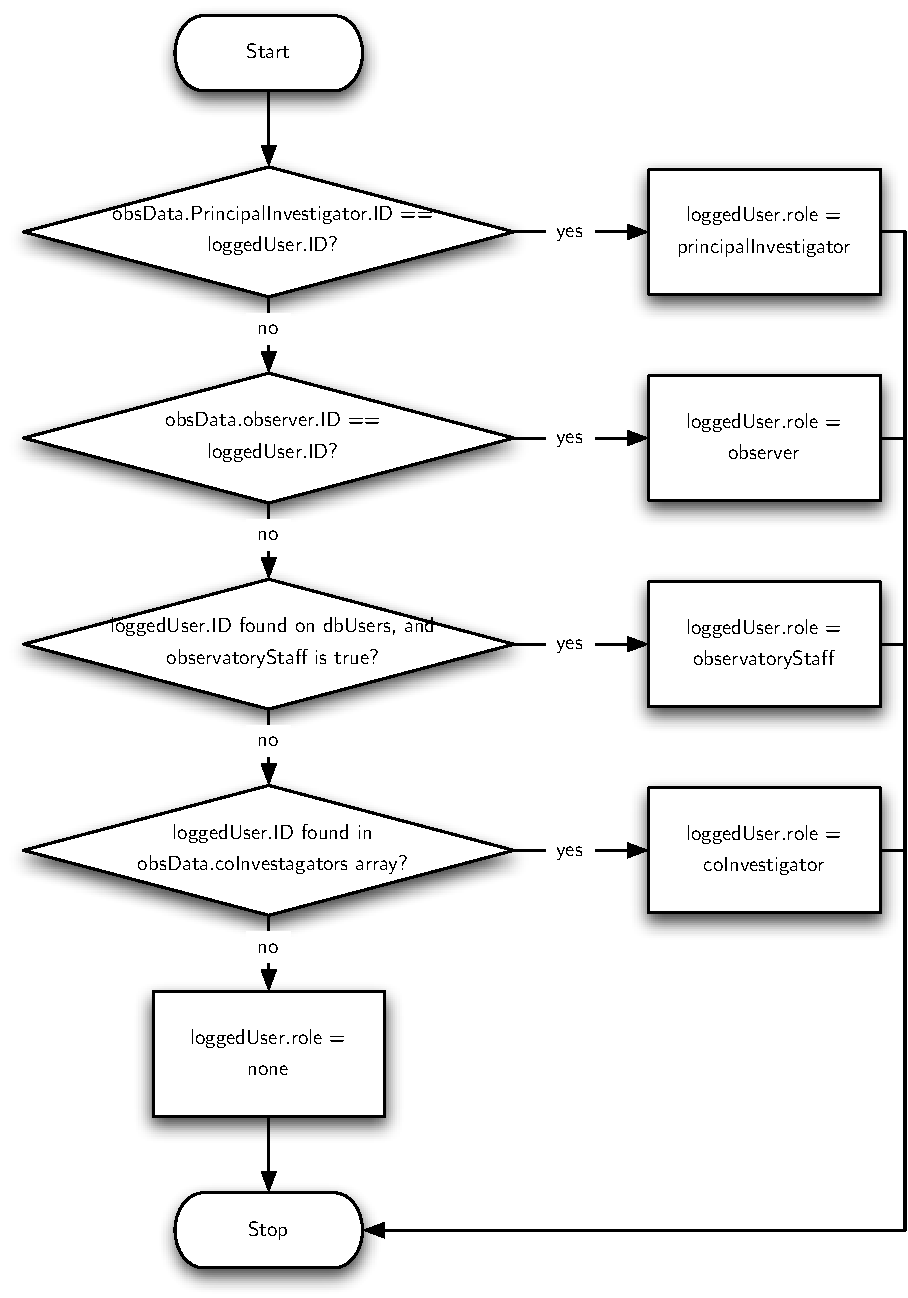
\includegraphics[width=\columnwidth]
			{fig/Policy-RoleDeterminationAlgorithm.pdf}
		\end{center}
		\caption[Role determination algorithm]
			{Flow diagram for the role determination algorithm.}
		\label{figPolicyRoles}
		\end{figure}
			
		This could be easily changed into a role-enabling algorithm
		that enables different roles for the same user, and
		displays all the different roles the user can access. If
		this is not needed, we will stick to the proposed
		algorithm.
		
		
		\begin{table}
		\begin{minipage}{\linewidth}
		\caption[Policy metadata]{Policy metadata.}
		\begin{smallertabular}{p{2.0 cm}p{1.25cm}p{3.6cm}p{4.4cm}}
				& \textbf{FITS} & & \\ \textbf{Attribute} & \textbf{Keyword} &
		        \textbf{UCD} & \textbf{Description}\\ \midrule projectID &
		        \texttt{PROJID} & \texttt{meta.curation.project;
		        meta.id}\footnote{There is no \texttt{meta.curation.project}
		        UCD, but we propose the inclusion of one.} & Project
		        identifier.\\ \addlinespace roleKind & \texttt{assign} &
		        \texttt{meta.policy.role; meta.code; meta.id}\footnote{There
		        are no \texttt{meta.policy.*} UCDs, but we propose, at least,
		        the inclusion of the \texttt{meta.policy} atom.} & Role kind
		        for which permissions will be provided.\\ \addlinespace permissions &
		        \texttt{assign} & \texttt{meta.policy.permissions;
		        meta.code}$^a$ & Permissions provided for roleKind users of
		        this project. The particular permissions to be provided are to
		        be discussed by IVOA.\\ \addlinespace
		\end{smallertabular}
		\label{tabPolicyMetadata}
		\end{minipage}
		\end{table}
		
		\begin{table}
		\begin{minipage}{\linewidth}
		\caption[Policy related Users metadata]{Policy related Users metadata.}
		\begin{smallertabular}{p{2.15 cm}p{1.5cm}p{2.35cm}p{5.25cm}}
				& \textbf{FITS} & & \\ \textbf{Attribute} & \textbf{Keyword} &
		        \textbf{UCD} & \textbf{Description}\\ \midrule
				
				userID & \texttt{COMMENT} & \texttt{meta.id} & User identifier
		        for all user related operations in the archive. \\ \addlinespace name
		        & \texttt{COMMENT} & \texttt{meta.name} & Real name of the
		        user. Any known user of the archive has to be registered, or be
		        anonymous. \\ \addlinespace institution & \texttt{COMMENT} &
		        \texttt{meta.name} & Name of the institution to which the user
		        belongs. \\ \addlinespace contactInfo & \texttt{COMMENT} &
		        \texttt{meta.note} & Contact info (probably e-mail) for this
		        user. \\ \addlinespace
		\end{smallertabular}
		\label{tabPolicyUsersMetadata}
		\end{minipage}
		\end{table}
		
		\begin{table}
		\begin{minipage}{\linewidth}
		\caption[Policy related Project metadata]
			{Policy related Project metadata.}
		\begin{smallertabular}{p{2.65 cm}p{1.5cm}p{3.3cm}p{3.80cm}}
				& \textbf{FITS} & & \\ \textbf{Attribute} & \textbf{Keyword} &
		        \textbf{UCD} & \textbf{Description}\\ \midrule projectID &
		        \texttt{PROJID} & \texttt{meta.curation.project;
		        meta.id}\footnote{There is no \texttt{meta.curation.project}
		        UCD, but we propose the inclusion of one.} & Project
		        identifier.\\ \addlinespace principalInvestigator & \texttt{COMMENT} &
		        \texttt{meta.id} & User identifier for the
		        principalInvestigator of the project. \\ \addlinespace
		        coInvestigator[n] & \texttt{COMMENT} & \texttt{meta.id} & User
		        identifier for the n\thsup\ co-investigator.\\ \addlinespace
		        title & \texttt{COMMENT} & \texttt{meta.curation.project;
		        meta.title}$^a$ & Project title.\\ \addlinespace description &
		        \texttt{COMMENT} & \texttt{meta.curation.project;
		        meta.note}$^a$ & Project description.\\ \addlinespace
		\end{smallertabular}
		\label{tabPolicyProjectMetadata}
		\end{minipage}
		\end{table}
		
		\begin{table}
		\begin{minipage}{\linewidth}
		\caption[Policy related DataID metadata]
			{Policy related DataID metadata.}
		\begin{smallertabular}{p{2.65 cm}p{1.5cm}p{3.3cm}p{3.80cm}}
				& \textbf{FITS} & & \\ \textbf{Attribute} & \textbf{Keyword} &
		        \textbf{UCD} & \textbf{Description}\\ \midrule projectID &
		        \texttt{PROJID} & \texttt{meta.curation.project;
		        meta.id}\footnote{There is no \texttt{meta.curation.project}
		        UCD, but we propose the inclusion of one.} & Project
		        identifier.\\ \addlinespace observationID & \texttt{OBSID} &
		        \texttt{obs; meta.dataset; meta.id} & User identifier for the
		        principalInvestigator of the project. \\ \addlinespace
		        coInvestigator[n] & \texttt{COMMENT} & \texttt{obs; meta.id} &
		        User identifier for the n\thsup\ project co-investigator.\\
		        \addlinespace title & \texttt{COMMENT} &
		        \texttt{meta.curation.project; meta.title}$^a$ & Project
		        title.\\ \addlinespace description & \texttt{COMMENT} &
		        \texttt{meta.curation.project; meta.note}$^a$ & Project
		        description.\\ \addlinespace creator & \texttt{AUTHOR} &
		        \texttt{meta.curation; meta.id} & User identifier for the
		        creator of the data entry.\\ \addlinespace observerID &
		        \texttt{OBSERVER} & \texttt{obs.observer; meta.id} & User
		        identifier for the person performing the observation producing
		        this data entry.\\ \addlinespace operatorID & \texttt{OBSERVER} &
		        \texttt{obs.operator; meta.id}\footnote{We propose the
		        inclusion of either \texttt{obs.operator} or
		        \texttt{instr.operator} as new UCDs to characterise
		        operator-related data. However, \texttt{obs.observer} can be
		        used when providing both observer and operator at the same
		        time.} & User identifier for the person performing operator
		        duties while performing the observation.\\ \addlinespace date &
		        \texttt{DATE-OBS} & \texttt{time.obs.start} & Date of
		        observation.\\ \addlinespace facility & \texttt{TELESCOP} &
		        \texttt{instr.obsty} & Facility (observatory) where the
		        telescope/instrument resides in.\\ \addlinespace instrument &
		        \texttt{INSTRUME} & \texttt{instr.tel} & Instrument performing
		        the observation\footnote{We have to study whether this should
		        contain an instrument-backend pair, or have different
		        attributes for both.}.\\ \addlinespace
		\end{smallertabular}
		\label{tabPolicyDataIDMetadata}
		\end{minipage}
		\end{table}
		

	% section policy (end)
	
	\section{Packaging} % (fold)
	\label{sec:packaging_the_vopack}
		
		\attributedquote{
			\dictionarydef
				{packaging}
				{noun}
				{
					\begin{itemize}
						\item materials used to wrap or protect
						goods.
						
						\item the business or process of packing
						goods.
						
						\item the presentation of a person,
						product, or action in a particular way.
					\end{itemize}
				}
		}
		{The New  Oxford American Dictionary, \emph{2nd Edition}}
		
		Digital data are usually thought of as free of \emph{bit
		rot}: digital copies are always bit perfect, but that is
		so because a lot of care is put into providing enough
		redundancy on the storage and interchange processes, so that
		possible bit flips can be detected and corrected.
		
		But changes in content can also be produced on
		intermediate states for a dataset: imagine reduced data
		products for which the calibration has been changed,
		producing at the same time a change in characterisation.
		The new data product being provided might link to an
		updated data product, but its characterisation can be
		the old one. Thus, we need a way to provide a permanent
		set of data products, which can be easily combined without
		further service queries by means of attached
		characterisation instances.
		
		\invisiblenote{
			\textbf{Rewrite this text coming from the DEA, both
			the Details chapter and VOPack appendix.}}
			
			The Packaging class is used to specify how data from
			different sources will be presented together. For
			instance, if we wanted to retrieve data belonging to
			our already mentioned maser survey, a VO system could
			reply with a Multi-Beam FITS file containing all the
			scans and sub-scans that conform the On-Off patterns for
			a single issued observation, or with a \texttt{.zip}
			file with all the FITS files belonging to the survey,
			or with just a single On-Off pair, et cetera.
			
			 An instance of the Packaging class would describe the
			contents of the data retrieved, in terms of project
			organisation, and of the particular files being
			actually delivered.
			
			 Unfortunately, there is no Packaging class defined at
			the VO level, so we have to resort to other packaging
			description mechanisms available in other archiving
			tools.
			
			First, we have to state the requirements for this class:
			
			\begin{itemize}
				\item The Packaging class will describe the type of
				compression or grouping, if any, applied to the
				result of a query. So, possible results should form
				a controlled vocabulary, such as \texttt{FITS},
				\texttt{VOTable}, \texttt{zip}, \texttt{tar},
				\texttt{gz}, \texttt{bz}, \texttt{bz2},
				\texttt{tgz}, \texttt{tbz}, \texttt{tbz2},
				corresponding to: raw files ---a FITS file or a
				VOTable---, a zip file, a tar file, a raw file
				compressed by gzip, bzip, bzip2, and a gzipped,
				bzipped or bzipped2 tar file.
				
				 \item We believe a standard VO packaging scheme is
				needed in order to facilitate distribution. We
				propose one such scheme, that we call VOPack
				---Virtual Observatory Package; \texttt{.vopack}
				file extension---. We will define the VOPack as a
				“tarred and gzipped” folder (\texttt{.tgz} file)
				with an XML content descriptor, which acts as
				VO-aware manifest of contained assets.
			\end{itemize}
			
			The VOPack is a way of distributing VO-compliant
			content, in a way that makes it easy to reuse and point
			to existing content, either remote or locally.
			
			A VOPack consists of a compressed file that contains at
			least a \texttt{voPack.xml} file —following the VOPack
			XML Schema— that describes all the additional content
			of the compressed VOPack, and their relationships
			between them. Figure~\ref{figVOPackStructure} shows the
			structure diagram of a VOPack.
			
			\begin{figure}[tbp]
			\begin{center}
				%\includegraphics[scale=1]{VOPackStructure.pdf}
				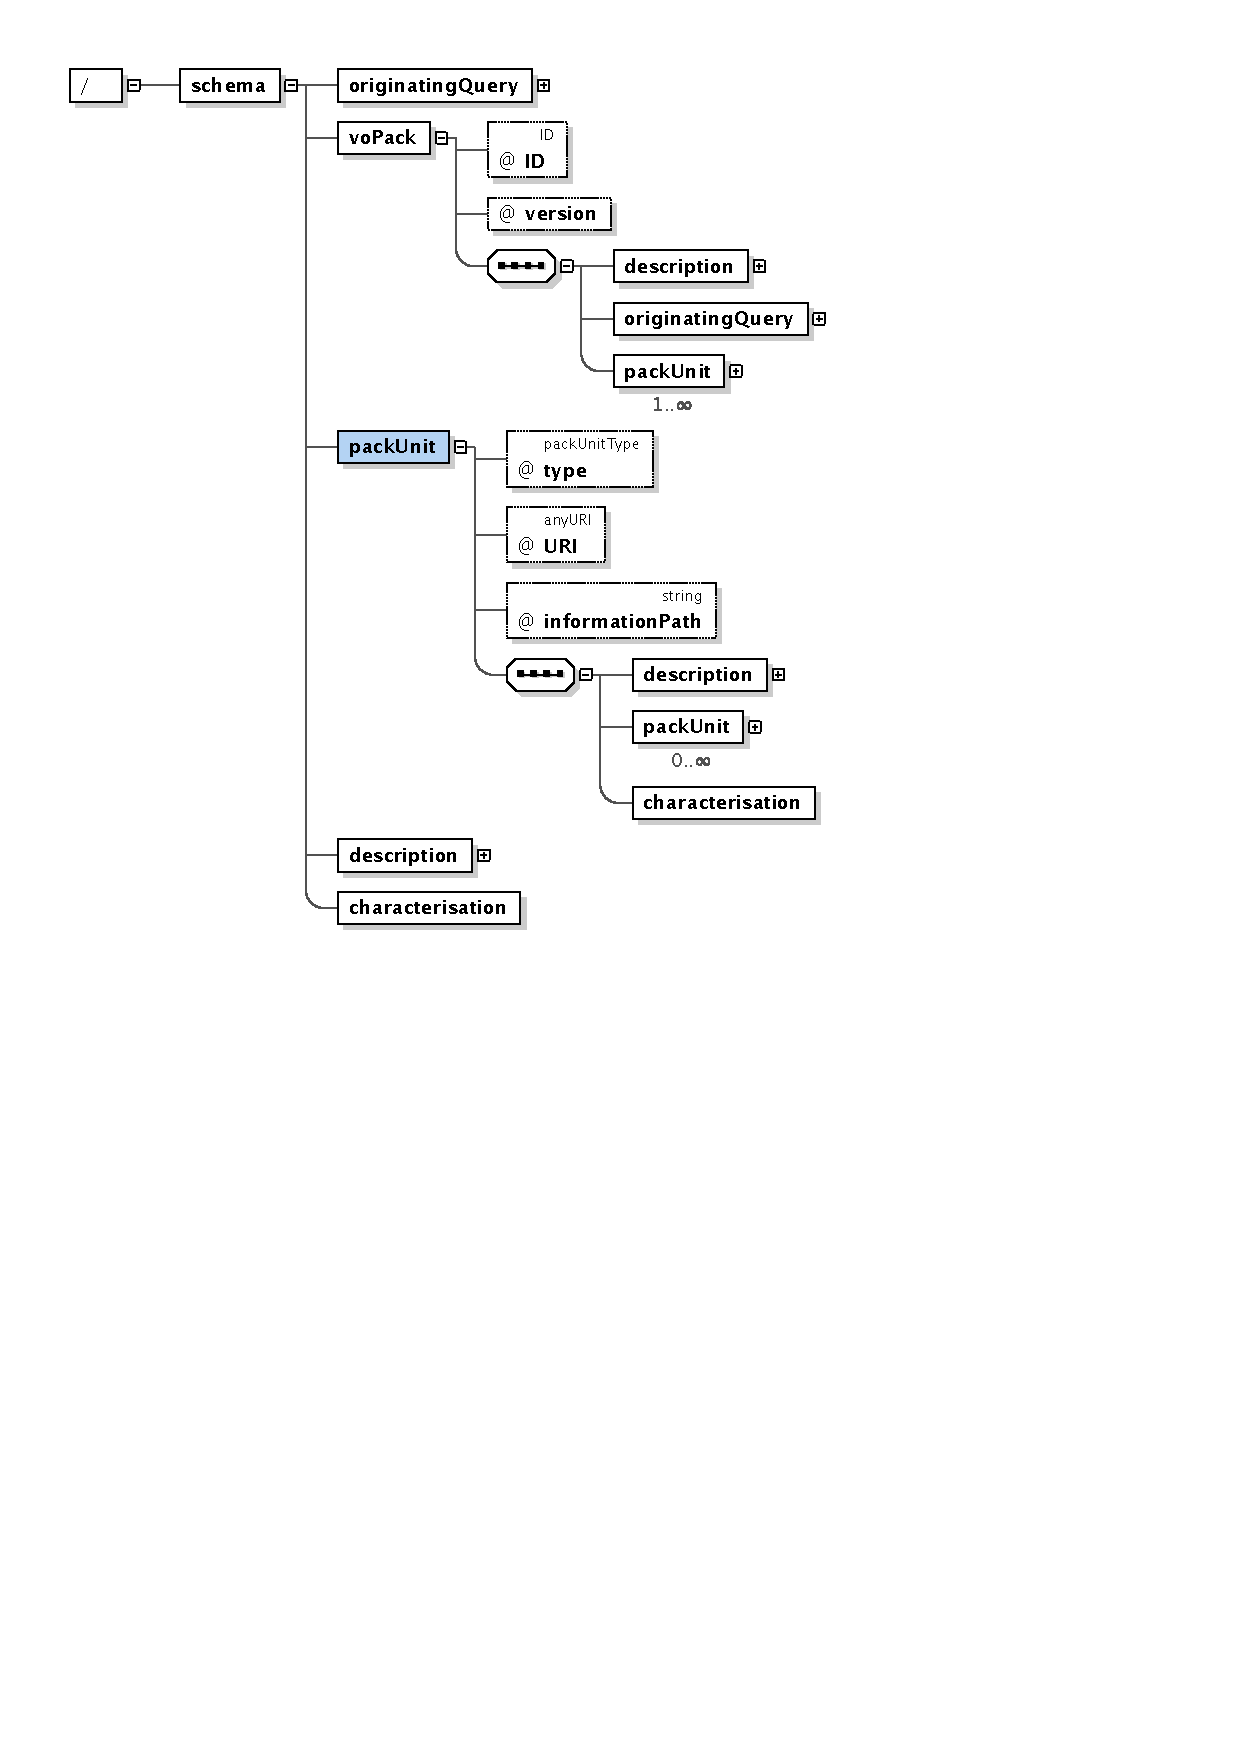
\includegraphics[scale=0.5]
				{fig/vopack-structure.pdf}
			\end{center}
			\caption[VOPack structure]
			{
				VOPack structure. Diagram generated by
				\textbf{Oxygen} from the XML schema.
			}
			\label{figVOPackStructure}
			\end{figure}
			
			In that diagram, the \texttt{voPack} element is the
			root for the XML document. It includes a description,
			the originating query, and one or more
			\texttt{packUnits}, which actually point to the
			information being retrieved. The
			\texttt{o\-rig\-i\-na\-ting\-Que\-ry}
			element contains the string
			with the URI that allows the retrieval of the voPack.
			Additional \texttt{characterisation} elements,
			following the Characterisation schema, can be used to
			further specify properties on the data being delivered
			with the VOPack.
			
			The \texttt{packUnit} corresponds to a single piece of
			data, or to another \texttt{packUnit}s, in case of more
			structured data. The depth of inclusion is arbitrary.
			
			\texttt{packUnit}s have a \texttt{type} attribute that
			can be one of:\texttt{votable}, \texttt{fits},
			\texttt{vopack}, \texttt{compressedFolder},
			\texttt{folder}, \texttt{otherXML},
			\texttt{otherNonXML}. Table~\ref{packUnitType}
			specifies the meaning of this attribute.
			
			\begin{table}
				\caption[Valid \texttt{packUnit} attribute values]{
					Meaning of the different valid values for
					attributes of the
					\texttt{packUnit} data type.
				}
				\begin{smalltabular}{rp{9.75cm}}
					\textbf{packUnit} &- \textbf{Description}
					\\\midrule
					
					 \texttt{votable} & The packed unit is a
					VOTable. \\\addlinespace
					
					 \texttt{fits} & The packed unit is a FITS
					file. \\\addlinespace
					
					 \texttt{vopack} & The packed unit is itself a
					VO pack. The characterisation of the
					referencing VO pack encompasses all packed
					units, while each particular one will have its
					own, \emph{narrower} characterisation.
					\\\addlinespace
					
					 \texttt{compressedFolder} & The referenced
					packed unit is a compressed directory.
					\\\addlinespace
					
					 \texttt{folder} & The referenced packed unit
					is a directory in the same file-system as the
					referencing VOPack. \\\addlinespace
					
					 \texttt{otherXML} & An XML representation,
					other than a VOTable, is used. \\\addlinespace
					
					 \texttt{otherNonXML} & A non-XML
					representation, also different from a FITS
					file, is used. This kind of representation
					should be avoided, but would be useful for
					packing instrument specific raw data formats,
					which are correctly characterised.
					\\\addlinespace \end{smalltabular}
					\label{packUnitType}
			\end{table}
			
			For the \texttt{vopack}, \texttt{folder} and
			\texttt{compressedFolder} values, a new
			\texttt{vopack.xml} file has to be provided for their
			description. This allows for meta-packaging of
			ready-made VOPacks.
			
			 For the first three types, the
			\texttt{informationPath} attribute gives an XPath to
			the actual data being pointed, just in case the
			\texttt{packUnit} contains several tables, and not all
			of them are to be considered. In the case of FITS
			files, the informationPath looks XPath-like, but points
			to the HDU or Image holding the data.
			
			 Figure~\ref{figVOPackXSDfile} shows the complete
			listing for the VOPack XML Schema.
			
			\begin{figure}[tbp]
			\begin{center}
				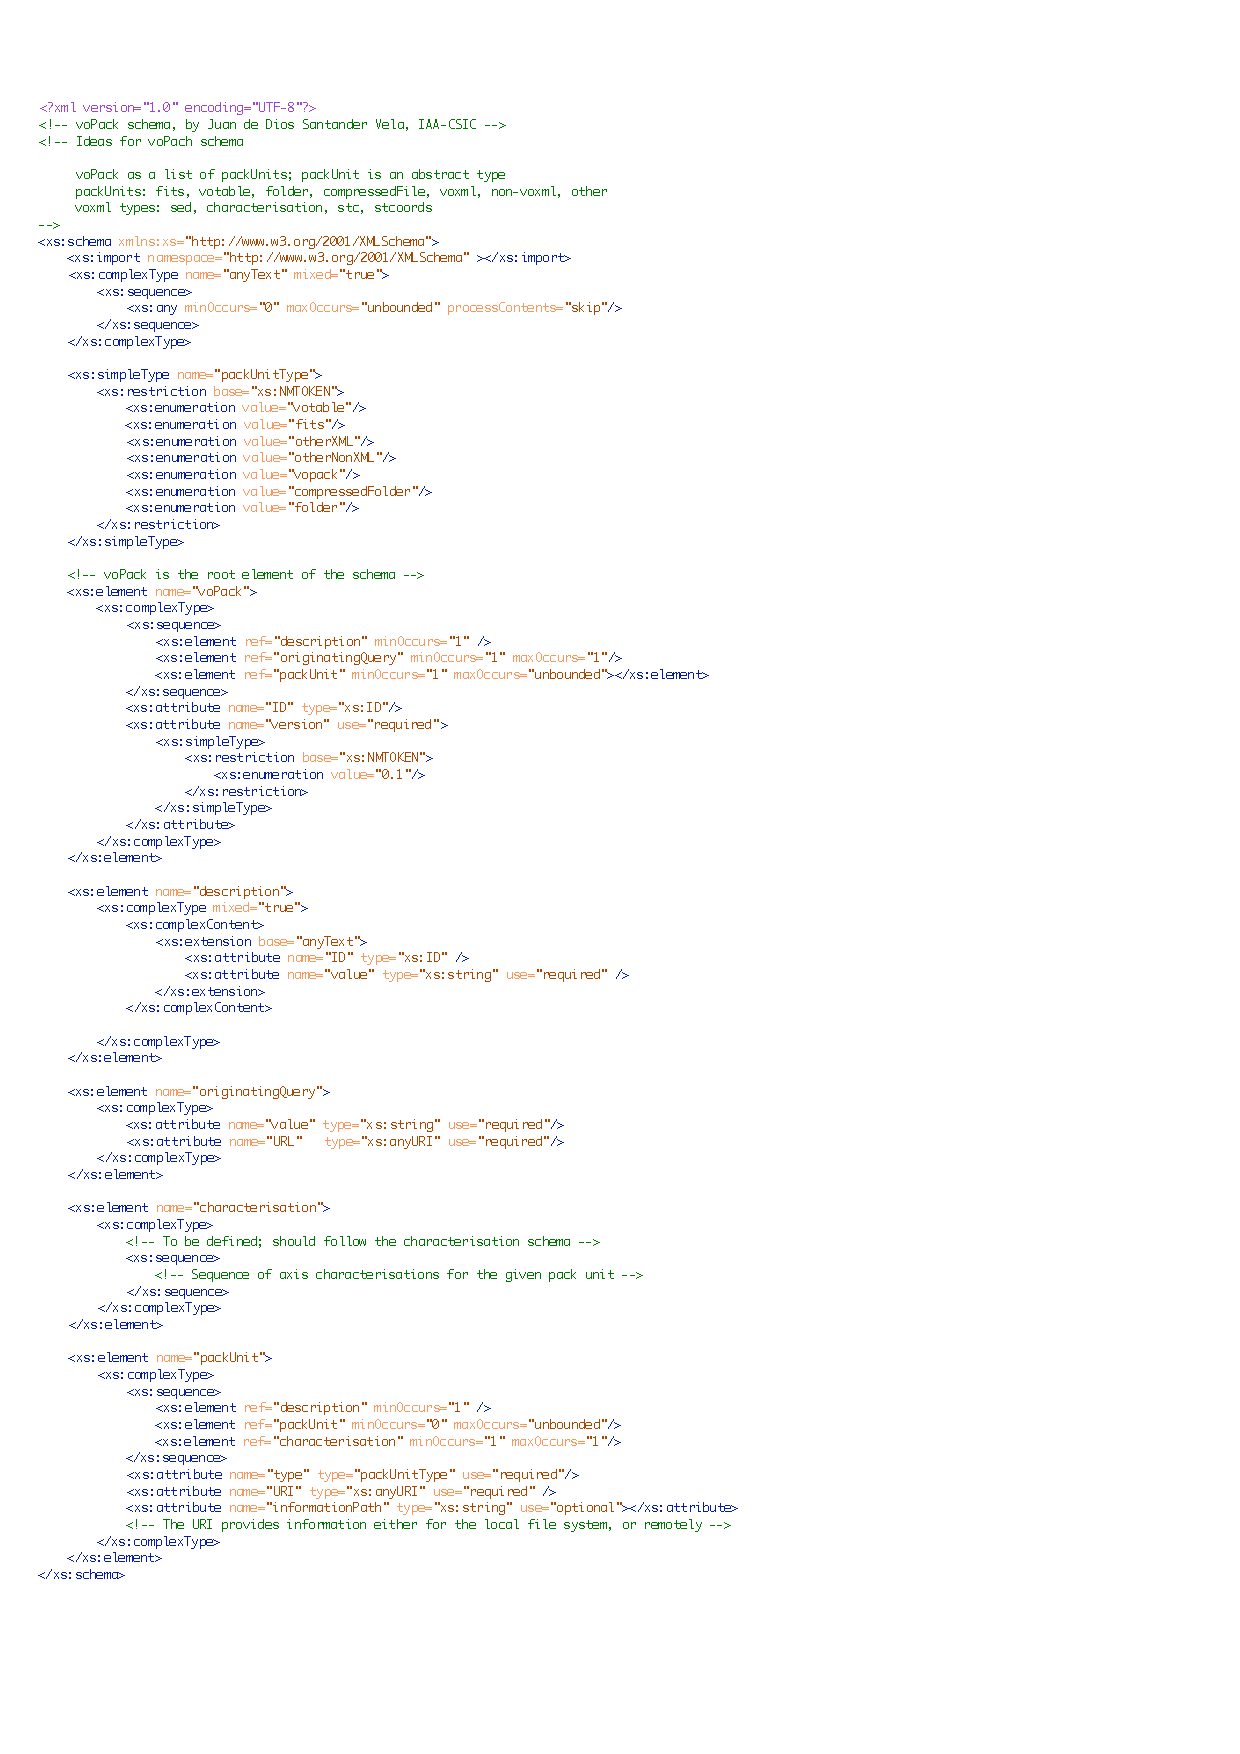
\includegraphics[totalheight=1\textheight]
				{fig/vopack-schemaListing.pdf}
			\end{center}
			\caption[VOPack schema listing]
			{VOPack XSD schema listing.}
			\label{figVOPackXSDfile}
			\end{figure}
			
			The VOPack XML Schema has been inspired by the concepts
			of Digital Items, Digital Item Containers, and Digital
			Item Components from MPEG-21~\cite{Bormans:fk}.
		
		
	% section packaging_the_vopack (end)
	
	\section{Conclusions} % (fold)
	\label{sec:radams_curation_etc_conclusions}
		
		In this chapter we have dealt with generic astronomical
		concepts, non-specific of radio astronomy, but which 
		were needed both for implementing the suggested ObsDM
		entities, but also for being able to successfully use IVOA
		data models as blueprints for archive development, as it
		will be shown when applying the data model to the archives
		of DSS-63 and IRAM~30m in
		chapter~\ref{cha:radams_based_archives}.
		
	% section radams_curation_etc_conclusions (end)
	
% chapter radams_curation_packaging_and_policy (end)